\chapter{Monte Carlo Simulation}\index{Monte Carlo simulation}

In 1946, the mathematician Stanislaw Ulam was recovering from an illness and
playing solitaire to pass the time. He wondered: what is the chance that a game
can be won? The combinations were far too many to count. Then he had a better
idea: just deal out a hundred games and see what fraction come out. With the new
electronic computers, you could deal out a million.

Ulam and his colleague John von Neumann named the idea after the famous casino in
Monte Carlo, and used it to design nuclear reactors. Today, \newterm{Monte Carlo
simulation} forecasts hurricanes, prices stock options, tests new medicines,
lights the scenes in animated movies, and helps sports websites predict who will
win the playoffs. The idea fits in one sentence:

\begin{center}
\emph{If you cannot calculate a probability, run the experiment many times on a computer, and count.}
\end{center}

In the Paradoxes chapter, you met two famous puzzles, the Monty Hall problem and
the birthday problem. In this chapter, you will settle them by experiment, and then
ask questions about them that are hard to answer any other way.

\section{Random Numbers in Python}
Python's built-in \texttt{random} library supplies the randomness:
\begin{itemize}
\item \mintinline{python}{random.random()} returns a number between 0 and 1, with every
value equally likely.
\item \mintinline{python}{random.randrange(n)} returns a whole number from 0 to $n - 1$.
\item \mintinline{python}{random.randint(a, b)} returns a whole number from $a$ to $b$,
including both.
\item \mintinline{python}{random.choice(items)} picks one item from a list.
\end{itemize}
Computers cannot really flip coins. These numbers come from a formula that produces
a long, unpredictable-looking sequence, so they are called \newterm{pseudorandom}. That
has a handy side effect: \mintinline{python}{random.seed(1)} restarts the sequence at
the same place, so a program gives the same ``random'' results every time it runs.
That is why you can check your output against this book.

\textbf{Why does counting work?} If an event has probability $p$, then in $n$
independent trials it happens about $pn$ times, so the fraction of successes is about
$p$. The more trials you run, the closer that fraction tends to get. This is the
\index{Law of Large Numbers}\newterm{Law of Large Numbers}. You will meet it again in the Limits chapter
(Volume 17), where it helps explain what a limit is.

\section{Estimating $\pi$ with Darts}\index{pi!Monte Carlo estimate}
Throw darts at a 1-by-1 square, completely at random. The square contains a quarter
of a circle of radius 1, with area $\frac{\pi}{4}$. Since the square has area 1, the
fraction of darts landing inside the quarter circle should be about $\frac{\pi}{4}$.
Multiply that fraction by 4, and you have an estimate of $\pi$.

A dart at $(x, y)$ is inside the quarter circle when its distance from the corner is
at most 1, that is, when $x^2 + y^2 \leq 1$.

\begin{figure}[H]
\centering
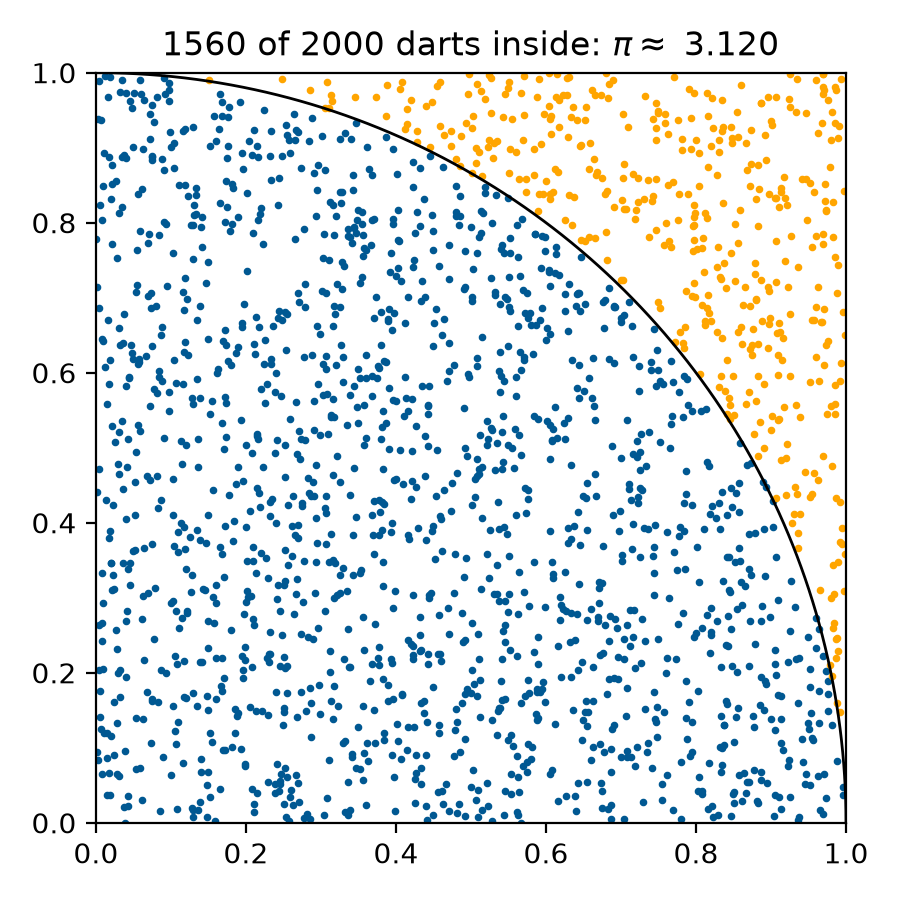
\includegraphics[width=0.5\textwidth]{darts.png}
\caption{Random darts. The blue ones landed inside the quarter circle.}
\label{fig:darts}
\end{figure}

\begin{minted}{python}
import random
import math

random.seed(1)                      # same "random" darts every run

def estimate_pi(darts):
    inside = 0
    for _ in range(darts):
        x = random.random()         # a random number from 0 to 1
        y = random.random()
        if x**2 + y**2 <= 1:        # inside the quarter circle?
            inside += 1
    return 4 * inside / darts

for darts in [100, 10_000, 1_000_000]:
    estimate = estimate_pi(darts)
    print(f"{darts:>9} darts: {estimate:.5f}  (error {abs(estimate - math.pi):.5f})")
\end{minted}
\begin{verbatim}
      100 darts: 3.20000  (error 0.05841)
    10000 darts: 3.13960  (error 0.00199)
  1000000 darts: 3.14118  (error 0.00042)
\end{verbatim}
A million random darts get $\pi$ right to about three decimal places. That is not
very precise (in Volume 33, infinite series will give you $\pi$ to as many digits as you
like), but this method used no math beyond the Pythagorean theorem.

\subsection{How Accurate Is a Simulation?}
Simulations are never exact, so you should always ask how far off yours might be. For
the dart estimate, a typical error is about $\frac{1.6}{\sqrt{n}}$ for $n$ darts:
about $0.16$ for 100 darts, $0.016$ for 10,000, and $0.0016$ for a million. (Our runs
happened to do a little better than typical.) The important part is the
$\sqrt{n}$: to get one more correct digit, you need 100 times as many trials. Monte Carlo
is easy to set up but slow to become precise. In Volume 30, you will learn to attach
exact margins of error to estimates like these.

\begin{Exercise}[title={Darts by Hand}, label=mc_darts]
You throw 400 darts and 312 land inside the quarter circle. What is your estimate of
$\pi$? About how many darts would you need to make the typical error 10 times smaller?
\end{Exercise}
\begin{Answer}[ref=mc_darts]
$\pi \approx 4 \cdot \frac{312}{400} = 3.12$. Since the error shrinks like $\frac{1}{\sqrt{n}}$,
making it 10 times smaller takes $10^2 = 100$ times as many darts: about 40,000.
\end{Answer}

\section{Monty Hall, the Whole Game}\index{Monty Hall Problem!simulation}
The simulation in the Paradoxes chapter used a shortcut: ``switching wins exactly when
your first pick was wrong.'' If you doubt the argument, you should doubt the shortcut
too. So here is the whole game, with a host who actually opens doors. The function
\mintinline{python}{play} works for any number of doors: the host opens every door
except your pick and one other, and he never reveals the car.

\begin{minted}{python}
import random

random.seed(2)

def play(switch, doors=3):
    car = random.randrange(doors)
    pick = random.randrange(doors)
    # The host opens every other door except one, never revealing the car.
    if pick == car:
        # any other door can stay closed
        closed = random.choice([d for d in range(doors) if d != pick])
    else:
        closed = car
    if switch:
        pick = closed
    return pick == car

games = 100_000
for switch in [False, True]:
    wins = sum(play(switch) for _ in range(games))
    print("switch" if switch else "stay  ", wins / games)
print("10 doors, switch:", sum(play(True, 10) for _ in range(games)) / games)
\end{minted}
\begin{verbatim}
stay   0.33293
switch 0.66468
10 doors, switch: 0.89813
\end{verbatim}
Staying wins about $\frac{1}{3}$ of the time and switching about $\frac{2}{3}$, just as
the Paradoxes chapter argued. The 10-door version makes the reason obvious: you pick 1
door, the host opens 8 goat doors, and the one door he deliberately leaves closed hides
the car 9 times out of 10.

\subsection{Monty Fall}
Here is a question that is easy to simulate and hard to argue about. Suppose the host
does \emph{not} know where the car is. He trips, and accidentally opens one of the two
doors you did not pick, at random. It happens to show a goat. Should you switch now?

\begin{minted}{python}
import random

random.seed(3)

kept = 0          # games where the host happened to show a goat
switch_wins = 0
for _ in range(100_000):
    car = random.randrange(3)
    pick = random.randrange(3)
    # The host slips and opens one of the other two doors at random.
    opened = random.choice([d for d in range(3) if d != pick])
    if opened == car:
        continue                       # car revealed: this game does not count
    kept += 1
    other = 3 - pick - opened          # the one remaining closed door
    if other == car:
        switch_wins += 1
print(kept, switch_wins / kept)
\end{minted}
\begin{verbatim}
66603 0.49958710568593007
\end{verbatim}
In about a third of the games, the clumsy host reveals the car, and we throw those games
out. In the rest, switching wins only half the time. The doors are the same, the goat
is the same, but the answer changed from $\frac{2}{3}$ to $\frac{1}{2}$. The advantage of
switching comes entirely from the host's \emph{knowledge}: a host who knows where the
car is and avoids it is giving you information. A host who reveals a goat by luck is
not.

\begin{Exercise}[title={Four Doors}, label=mc_four]
In a 4-door version, you pick a door, the host (who knows where the car is) opens one
goat door, and you switch to one of the two remaining closed doors at random. Write a
simulation to estimate your chance of winning. Then explain the answer.
\end{Exercise}
\begin{Answer}[ref=mc_four]
\begin{minted}{python}
import random

def four_doors():
    car = random.randrange(4)
    pick = random.randrange(4)
    goats = [d for d in range(4) if d != pick and d != car]
    opened = random.choice(goats)
    rest = [d for d in range(4) if d != pick and d != opened]
    return random.choice(rest) == car

games = 100_000
print(sum(four_doors() for _ in range(games)) / games)
\end{minted}
It prints about 0.375. Explanation: your first pick is wrong $\frac{3}{4}$ of the time.
Then the car is behind one of the two doors you might switch to, and you choose the
right one half the time: $\frac{3}{4} \cdot \frac{1}{2} = \frac{3}{8}$. That beats staying,
which wins only $\frac{1}{4}$.
\end{Answer}

\section{The Birthday Problem}\index{birthday problem!simulation}
In the Paradoxes chapter, a product formula showed that 23 people have a better than
even chance of a shared birthday. A simulation checks it without any formula: fill a
room with random birthdays and see whether any repeat. A Python \texttt{set} keeps only
one copy of each value, so the room has a repeat exactly when the set is smaller than
the list.

\begin{minted}{python}
import random

random.seed(4)

def shared_birthday(people, trials=20_000):
    hits = 0
    for _ in range(trials):
        birthdays = [random.randrange(365) for _ in range(people)]
        if len(set(birthdays)) < people:   # a set drops repeats
            hits += 1
    return hits / trials

def exact(people):
    no_match = 1
    for i in range(people):
        no_match *= (365 - i) / 365
    return 1 - no_match

for n in [10, 23, 30, 50]:
    print(f"{n} people: simulated {shared_birthday(n):.3f}, exact {exact(n):.3f}")
\end{minted}
\begin{verbatim}
10 people: simulated 0.121, exact 0.117
23 people: simulated 0.505, exact 0.507
30 people: simulated 0.712, exact 0.706
50 people: simulated 0.970, exact 0.970
\end{verbatim}

\begin{figure}[H]
\centering
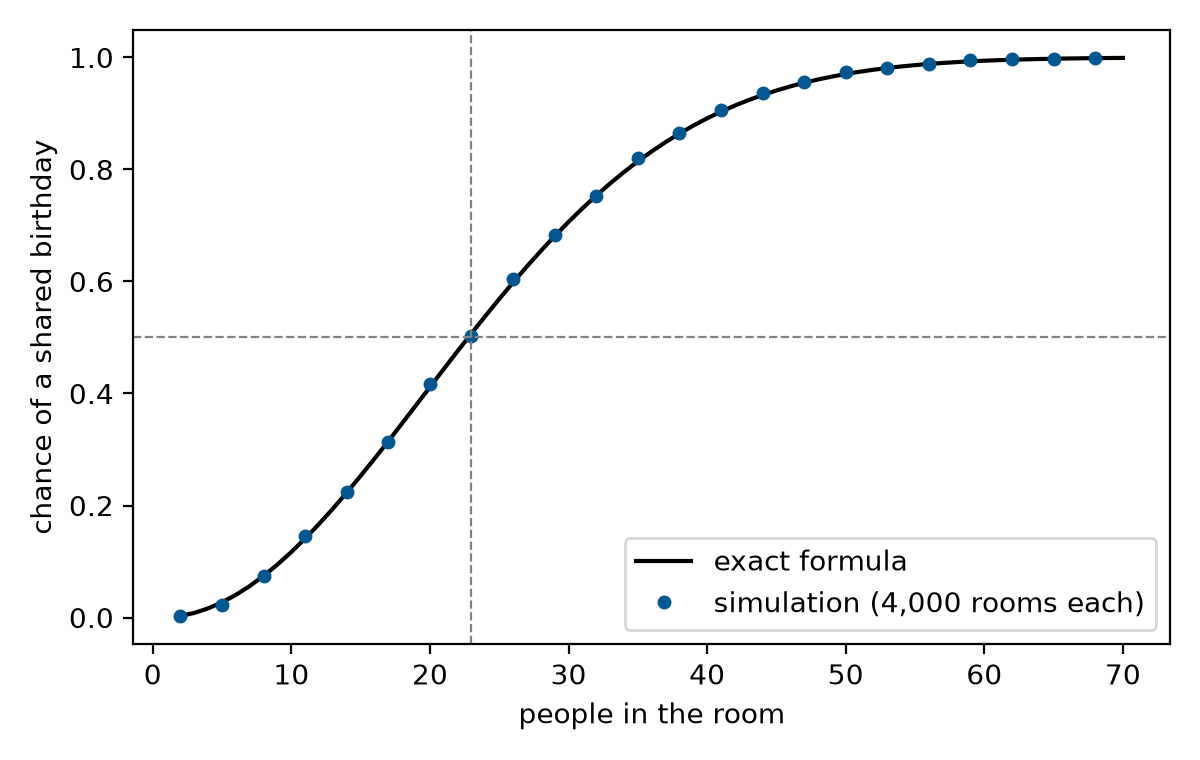
\includegraphics[width=0.75\textwidth]{birthday.png}
\caption{Simulated rooms (dots) match the exact formula (curve). The dashed lines
cross at 23 people and a 50\% chance.}
\label{fig:birthday}
\end{figure}

\subsection{A Question Without a Formula}
Here is where simulation shines. How many people do you need for a better than even
chance that \emph{three} of them share a birthday? The neat product formula no longer
works, because there are many ways for birthdays to overlap. But the simulation needs
only a small change: count how many people have each birthday, and look for a day with
three or more. Python's \texttt{Counter} does the counting.

\begin{minted}{python}
import random
from collections import Counter

random.seed(5)

def triple_birthday(people, trials=10_000):
    hits = 0
    for _ in range(trials):
        counts = Counter(random.randrange(365) for _ in range(people))
        if max(counts.values()) >= 3:      # some day has 3 or more people
            hits += 1
    return hits / trials

for n in [23, 50, 80, 88, 100]:
    print(n, triple_birthday(n))
\end{minted}
\begin{verbatim}
23 0.0129
50 0.1274
80 0.4118
88 0.5157
100 0.6497
\end{verbatim}
The chance first passes 50\% at 88 people. Mathematicians have confirmed that number
with much harder exact calculations, but the simulation found it in half a second.

\begin{Exercise}[title={Lucky Seven}, label=mc_dice]
Simulate rolling two dice 100,000 times, and estimate the probability that the sum is 7.
Then find the exact answer by listing all 36 equally likely outcomes.
\end{Exercise}
\begin{Answer}[ref=mc_dice]
\begin{minted}{python}
import random

rolls = 100_000
sevens = sum(random.randint(1, 6) + random.randint(1, 6) == 7 for _ in range(rolls))
print(sevens / rolls)
\end{minted}
It prints about 0.167. Exactly: the outcomes (1,6), (2,5), (3,4), (4,3), (5,2), and
(6,1) give 7, so the probability is $\frac{6}{36} = \frac{1}{6} \approx 0.1667$.
\end{Answer}

\begin{Exercise}[title={Two Heads in a Row}, label=mc_hh]
You flip a fair coin until you get two heads in a row. On average, how many flips does
it take? Write a simulation to estimate the answer.
\end{Exercise}
\begin{Answer}[ref=mc_hh]
\begin{minted}{python}
import random

def flips_until_hh():
    flips = 0
    previous_heads = False
    while True:
        flips += 1
        heads = random.random() < 0.5
        if heads and previous_heads:
            return flips
        previous_heads = heads

trials = 100_000
print(sum(flips_until_hh() for _ in range(trials)) / trials)
\end{minted}
It prints a number close to 6. (The exact answer is 6, which you can prove with the
tools of the probability chapters.)
\end{Answer}

\begin{Exercise}[title={Area by Darts}, label=mc_area]
Change the dart program to estimate the area under the curve $y = x^2$ between
$x = 0$ and $x = 1$. (Count a dart as a hit when $y \leq x^2$.) What does the estimate
come out close to?
\end{Exercise}
\begin{Answer}[ref=mc_area]
Replace the test with \mintinline{python}{if y <= x**2:}, and report
\mintinline{python}{inside / darts} instead of multiplying by 4. With 100,000 darts,
the estimate is about 0.333. The exact area is $\frac{1}{3}$, as you will be able to
show with integrals in Volume 30. Using random points to estimate areas like this is
called \newterm{Monte Carlo integration}; for complicated shapes in many dimensions, it is
often the only practical method.
\end{Answer}

\begin{mdframed}[style=important, frametitle={Key Ideas}]
\begin{itemize}
\item Monte Carlo simulation estimates a probability by running a random experiment many times on a computer and counting how often the event happens.
\item Python's \texttt{random} library produces pseudorandom numbers, and \texttt{random.seed} makes a program repeat the same results.
\item By the Law of Large Numbers, the fraction of successes gets closer to the true probability as the number of trials grows.
\item Simulation error shrinks in proportion to $\frac{1}{\sqrt{n}}$, so each extra correct digit takes 100 times as many trials.
\item In the Monty Hall game, switching wins $\frac{2}{3}$ of the time because the host knows where the car is. A host who opens a door at random gives no advantage.
\item Simulation can answer questions that have no neat formula, such as how many people make a three-way shared birthday more likely than not (88).
\end{itemize}
\end{mdframed}
